\counterwithout{section}{chapter}
\section{Цель лабораторной работы}

Знакомство со средством дизассемблирования – sourcer и с получением дизассемблерного кода ядра операционной системы Windows на примере обработчика прерывания Int 8h в virtual mode – специальном режиме защищенного режима, который эмулирует реальный режим работы вычислительной системы на базе процессоров Intel.

\section{Задание}

Используя Sourser получить дизассемблерный код обработчика аппаратного прерывания от системного таймера INT 8h. На основе полученного кода составить алгоритм работы обработчика INT 8h.

\section{Листинги кода}

\lstinputlisting[style={asm}, caption=Листинг прерывания INT 8h]{../lst/INT8h.LST}

\lstinputlisting[style={asm}, caption=Листинг процедуры sub\_9]{../lst/SUB9.LST}

\section{Схемы алгоритмов}

\begin{figure}[h!]
	\begin{center}
		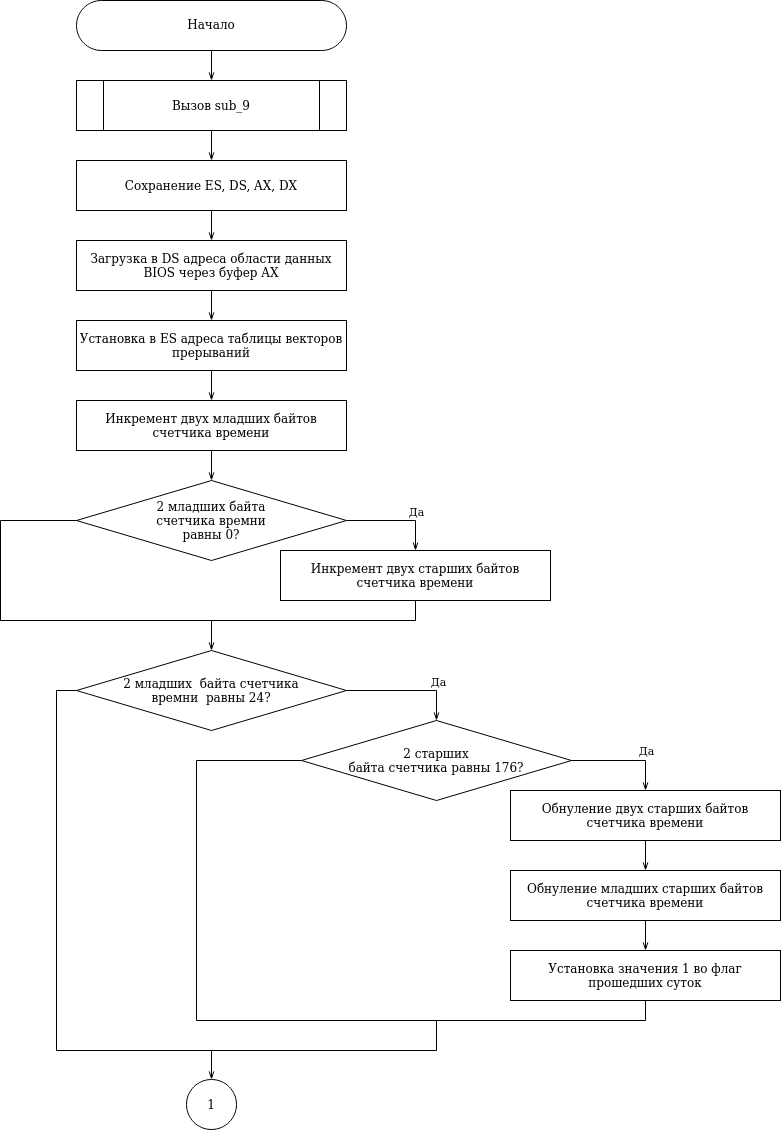
\includegraphics[scale=0.6]{assets/int8F.drawio.png}
		\caption{Схема алгоритма прерывания INT 8h}
	\end{center}
\end{figure}

\begin{figure}[h!]
	\begin{center}
		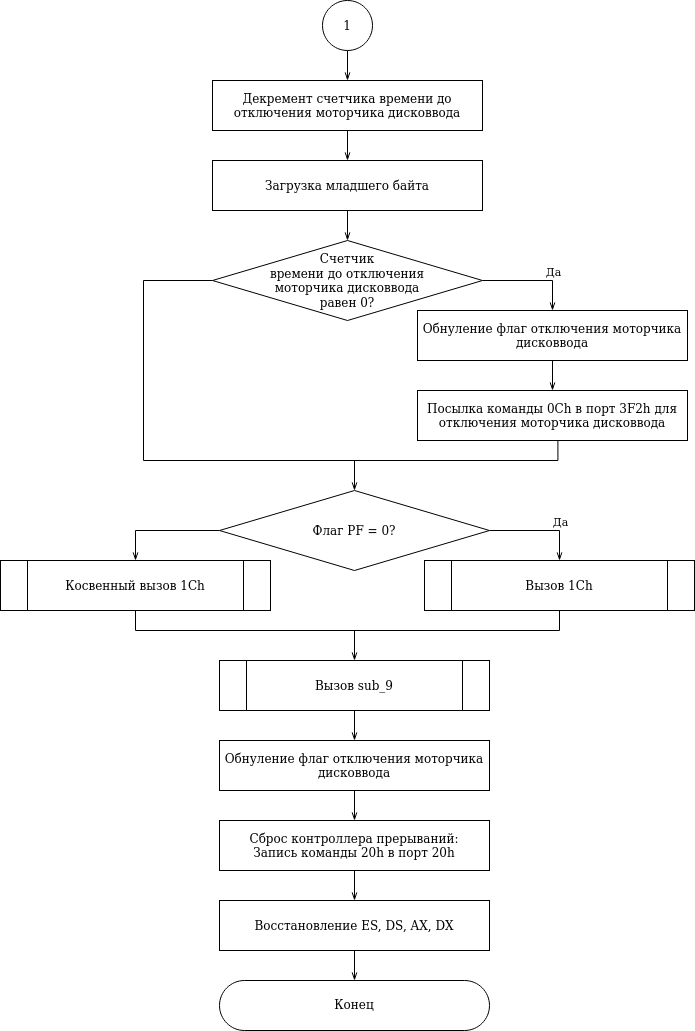
\includegraphics[scale=0.6]{assets/int8_1F.drawio.png}
		\caption{Схема алгоритма прерывания INT 8h}
	\end{center}
\end{figure}

\begin{figure}[h!]
	\begin{center}
		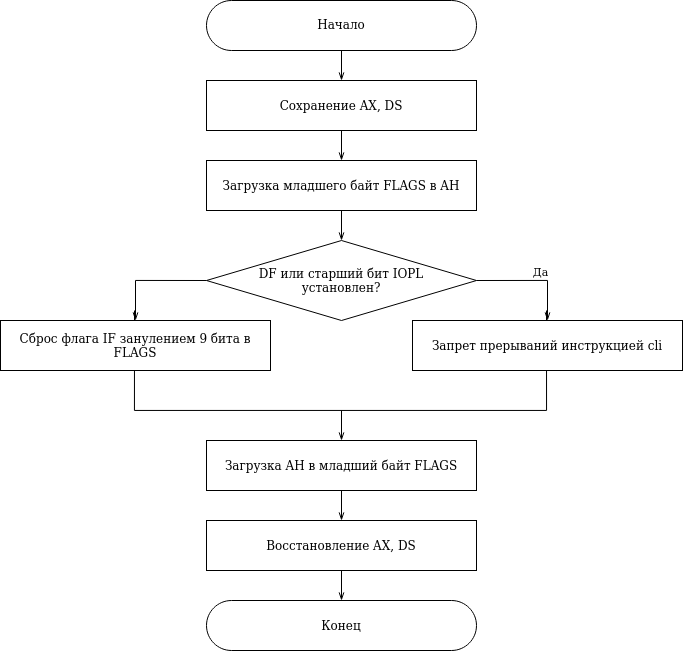
\includegraphics[scale=0.65]{assets/sub_9F.drawio.png}
		\caption{Схема процедуры sub\_9}
	\end{center}
\end{figure}